\documentclass[../poliXuniversity_hospital_(USP)_report.tex]{subfiles}
\graphicspath{ {images/}{../images/} }

\begin{document}
\chapter{Visão Computacional}

Por falta de tempo, ainda não foi possível dar continuidade às pesquisas que o João Pedro \cite{sotto_rel20} começou e implementar algo concreto no robô.

De maneira geral, como todo o grupos estava utilizando ROS para a produção de algoritmos de controle, as pesquisas sobre visão computacional foram em cima de ferramentas que facilitassem a comunicação com o ROS.

A princípio, além do OpenCV,  foi utilizado a ferramenta Darknet\cite{darknet21} e Darknet Ros \cite{darknetros21}, que já são grandes datas set com uma comunicação facilitada e pré estabelecida com ROS. De maneira geral os testes com essas ferramentas foram um sucesso nos computadores convencionais, como pode ser visto nas figuras ~\ref{fig:Teste de visão Computacional -  Simulação} e ~\ref{fig:Teste de visão Computacional -  Real}.

\begin{figure}[h]
\centering
    \caption{Teste de visão Computacional -  Simulação}
    \centering % para centralizarmos a figura
    \includegraphics[width=12cm]{visão_computacional_simulado.jpg}
    \caption*{Fonte: Elaborado pelo Autor no Software Gazebo \cite{gazebo21}}
    \label{fig:Teste de visão Computacional -  Simulação}
\end{figure}

\begin{figure}[h]
\centering
    \caption{Teste de visão Computacional -  Real}
    \centering % para centralizarmos a figura
    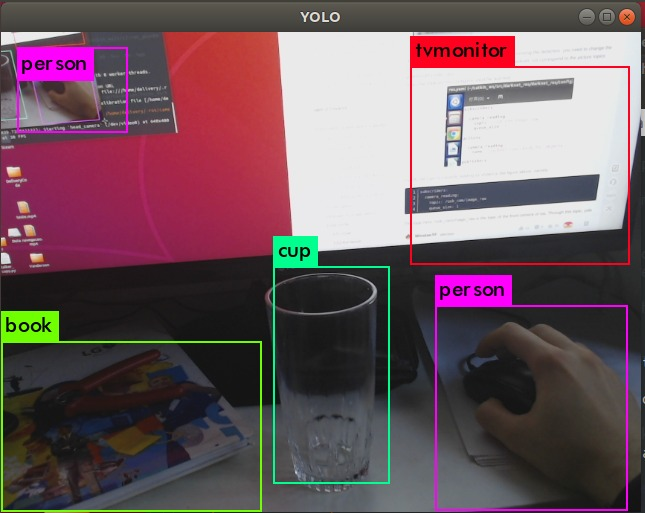
\includegraphics[width=12cm]{visao_computacional_real.jpg}
    \caption*{Fonte: Elaborado pelo autor}
    \label{fig:Teste de visão Computacional -  Real}
\end{figure}

Entretanto, os testes usando o computador embarcado, a Jetson Nano , não foram satisfatórios e a ideia acabou sendo deixada de lado para dar prioridade para outras áreas.

\end{document}